\part{A Framework with the Serializability Guarantee}

\chapter{The \hemiola{} Domain-Specific Language}
\label{sec-hemiola-dsl}

As explained in \autoref{sec-sz-def}, on top of serializability, it is much easier to design and prove invariants.
That being said, it will still be a large burden if a user has to prove serializability per-protocol.
In this chapter, we would like to provide \emph{abstract conditions} to prove serializability, in order not to prove it directly for each protocol.
Furthermore, we design a domain-specific language (DSL) that every protocol defined on top of this language automatically satisfies the conditions to guarantee serializability.
The conditions have already been mentioned with the motivating example in \autoref{sec-nutshell} -- network topology and locking mechanisms, extracted from transient states of practical cache-coherence protocols.

\section{Topology and Network Requirements}
\label{sec-topo-net-reqs}

In order to employ the serializability guarantee in \hemiola{}, the objects in a given system should form a tree topology.
Most cache-coherent memory subsystems follow this topology, where leaf nodes correspond to L1 caches, and the root corresponds to the main memory.
A child and its parent in the tree communicate using the three channels shown in \autoref{sec-nutshell}: an upward-request channel, an upward-response channel, and a single downward channel.
Note that the use of the three channels does not mean the actual hardware implementation should use just the three channels; it can use any channel implementation that refines the three channels regarded as a specification.
For example, we may want to have an additional queue that accepts all the requests from child caches (from the corresponding upward-request channels), so the parent can have a single entry point to handle child requests.
We will indeed see in \autoref{sec-comp-syn} how logical channels in \hemiola{} are implemented in a register-transfer level.

\hemiola{} as a Coq library generates the topology and network channels automatically from instances of a simple inductive type.
For example, the following tree definition will generate topology and channels for four L1 caches, two L2 caches, the last-level cache (LLC), and the main memory:
\begin{lstlisting}[numbers=none, frame=none]
  Definition t: tree := Node [Node [Node [Leaf; Leaf]; Node [Leaf; Leaf]]].
\end{lstlisting}

\section{Locking Mechanism}
\label{sec-locking-mechanism}

We saw in \autoref{sec-nutshell} why fine-grained transient states are required to ensure safe interleavings in cache-coherence protocols.
Revisiting the corner case described in \autoref{fig-motive-2}, a child should be able to handle an invalidation request from the parent even if it is in a transient state (SM), and after the response it changes its transient state to IM.
By looking at these transient states carefully, we have discovered that another necessary condition, other than the tree-topology condition, is the locking perspective from the transient states.

\hemiola{} supports a general locking mechanism reflecting this discovery;
instead of looking at the type of a message (\eg{} invalidation), the framework provides \emph{more-general} locking, just by looking at whether the message is from the parent or one of its children.
This relaxed locking mechanism is then not coupled with any specific cache-coherence protocols but is still sufficient to prove serializability.

\tikzset{
  uprightedge/.pic = {
    \draw [>->] (0.2, 0.25) -- (0.8, 1.05);
  },
}
\begin{figure}[h]
  \centering
  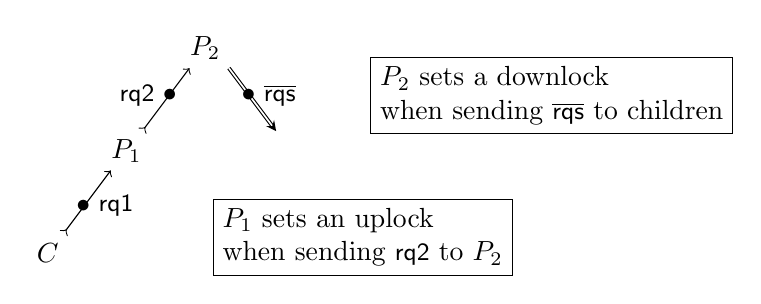
\begin{tikzpicture}
    \node at (0, 0) {$C$};
    \pic at (0, 0) {uprightedge};
    \node[label={[label distance=-4pt]right:{\small {\sf rq1}}}] at (0.45, 0.6) {$\bullet$};
    \node at (1.0, 1.3) {$P_1$};
    \pic at (1.0, 1.3) {uprightedge};
    \node[label={[label distance=-4pt]left:{\small {\sf rq2}}}] at (1.55, 2.0) {$\bullet$};
    \node at (2.0, 2.6) {$P_2$};

    \draw [>=stealth,double,->] (2.3, 2.35) -- (2.9, 1.55);
    \node[label={[label distance=-4pt]right:{\small $\overline{\textsf{rqs}}$}}] at (2.55, 2.0) {$\bullet$};

    \node[draw,align=left] at (4.0, 0.2) {$P_1$ sets an uplock\\ when sending {\small $\textsf{rq2}$} to $P_2$};
    \node[draw,align=left] at (6.4, 2.0) {$P_2$ sets a downlock\\ when sending {\small $\overline{\textsf{rqs}}$} to children};
  \end{tikzpicture}
  \caption{The uplock and downlock in \hemiola{}}
  \label{fig-locking}
\end{figure}

In particular, \hemiola{} provides two kinds of locks: \emph{uplocks and downlocks}.
We say an object is uplocked (or downlocked) when it holds an uplock (or downlock), respectively.
\autoref{fig-locking} depicts the locking mechanism in \hemiola{}.
An uplock is set when an object makes an upward request to its parent ($P_1$ in the figure); it is released when the object gets a corresponding response from the parent.
On the contrary, a downlock is set when an object makes a downward request(s) to some of its children ($P_2$ in the figure).

\begin{figure}[h]
  \centering
  \renewcommand{\arraystretch}{1.2}
  \newcommand{\lockyes}{\cmark}
  \newcommand{\lockno}{\xmark}
  \begin{tabular}{ccc}
    \hline
    & Uplocked & Downlocked\\
    \hline
    Acquiring an uplock & \lockno & \lockyes\\
    Releasing an uplock & \lockyes & \lockno\\
    Acquiring a downlock & \lockyes & \lockno\\
    Releasing a downlock & \lockyes & \lockyes\\
    \hline
  \end{tabular}
  \caption{Locking conditions in \hemiola{}}
  \label{fig-locking-conditions}
\end{figure}

\autoref{fig-locking-conditions} shows the conditions to acquire or release the locks.
An uplock can be set if the object is not yet uplocked; it can be set even when the object is downlocked.
This locking mechanism means that an object can make a request to the parent even when it has made requests to the children.
It is still safe, since the lock release will not be allowed when downlocked, \ie{} the uplock release should always wait for the downlock to be released.
On the other hand, a downlock \emph{can be set and released even when uplocked}.
This relaxation is very important to make the locking mechanism both safe and live.
If a downlock could not be released when uplocked, we would have a deadlock case, where the both locks wait for each other.

Now every cache object defined in \hemiola{} \emph{does not need to set transient states} to consider all combinations among stable statuses;
instead, the framework helps maintain the cache status and claim proper locks.
For example, instead of setting a transient state SM, it is now desirable to maintain its status S and to set an uplock to record it just made the upward request.
(The framework provides even more, actually, by guiding users to employ the \emph{rule templates}, introduced in the next section, that automatically set proper locks.)

Each object defined in \hemiola{} has a semantic \emph{lock state}, a finite map from a lock type (uplock or downlock) to lock information: the original request message, the original requestor index, and requestee indices from which we expect to get responses.
In the common terminology of cache-coherence protocols, each lock corresponds to a miss status holding register (MSHR).
An MSHR is set when a cache miss happens and the miss triggers further requests to obtain a proper status and up-to-date data.
As with \hemiola{} lock holders, MSHRs play a crucial role both in deciding whether to handle certain requests and in storing information needed to handle them properly.

It is worth emphasizing that an uplock and a downlock are assigned for each line.
In other words, the locking conditions presented in \autoref{fig-locking-conditions} do not apply to the locks for different cache lines.
This separation is safe, since in a cache-coherence protocol the transactions for different cache lines never interfere with each others.
It is not practical, however, to have an uplock and a downlock for each line in the actual hardware implementation.
We need to restrict the number of locks (MSHRs) to make the implementation synthesizable.
A detailed discussion about this restriction will be provided in \autoref{sec-comp-syn}.

\section{Rule Templates}
\label{sec-rule-templates}

\newcommand{\rtname}[1]{{\small\sf\bf #1}}

\newcommand{\uled}{\ensuremath{\textsf{UL}}}
\newcommand{\dled}{\ensuremath{\textsf{DL}}}
\newcommand{\ulfree}{\ensuremath{\textsf{UL}_{\times}}}
\newcommand{\dlfree}{\ensuremath{\textsf{DL}_{\times}}}

\newcommand{\setul}{\ensuremath{\textsf{UL}\Uparrow}}
\newcommand{\setdl}{\ensuremath{\textsf{DL}\Uparrow}}
\newcommand{\relul}{\ensuremath{\textsf{UL}\Downarrow}}
\newcommand{\reldl}{\ensuremath{\textsf{DL}\Downarrow}}
\newcommand{\stsilent}{\ensuremath{\textsf{SLT}}}

\newcommand{\ppo}[3]{\ensuremath{\{#1\}#2\lbrack#3\rbrack}}
\newcommand*{\bfrac}[2]{\genfrac{}{}{0pt}{}{#1}{#2}}

On top of the topology/network requirements and the locking mechanism, \hemiola{} provides rule templates to ensure that objects communicate within the topology and locks are properly set.
In this section, we will explore what kinds of rule templates \hemiola{} provides and discuss their uses.
Each rule template will be introduced with the form $\ppo{P}{O}{Q}$ and arrows with $\circ$ and $\bullet$, which means that the rule template is for an object $O$, requires input messages ($\circ$) and a precondition $P$, performs a state transition $Q$, and generates output messages ($\bullet$).
$\uled$, $\dled$, $\ulfree$, and $\dlfree$ in a precondition indicate that the object is uplocked, downlocked, uplock-free, and downlock-free, respectively.
$\setul$, $\setdl$, $\relul$, and $\reldl$ in a state transition indicate setting an uplock, setting a downlock, releasing an uplock, and releasing a downlock, respectively.
$\stsilent{}$ annotates that the rule template forbids any state modification beside locking.

\paragraph{Rule templates for immediate responses}

\begin{center}
  \begin{tabular}{p{0.18\textwidth}p{0.77\textwidth}}
    \begin{adjustbox}{valign=t}
      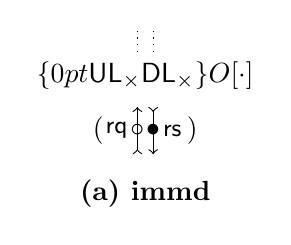
\begin{tikzpicture}
        \draw [dotted] (-0.1, 0.5) -- (-0.1, 0.8);
        \draw [dotted] (0.1, 0.5) -- (0.1, 0.8);
        \node at (0, 0.2) {$\ppo{\bfrac{\ulfree{}}{\dlfree{}}}{O}{\cdot}$};
        \draw [<-<] (-0.1, -0.2) -- (-0.1, -0.8);
        \draw [>->] (0.1, -0.2) -- (0.1, -0.8);
        \node[label={[label distance=-6pt]left:{\small {\sf rq}}}] at (-0.1, -0.5) {$\circ$};
        \node[label={[label distance=-6pt]right:{\small {\sf rs}}}] at (0.1, -0.5) {$\bullet$};
        \node at (0, -0.5) {$(\qquad\quad)$};
        \node at (0, -1.3) {{\bf (a) immd}};
      \end{tikzpicture}
    \end{adjustbox}&
    An immediate-down ({\bf immd}) rule responds immediately to an upward request, requiring the both locks free.
    This rule possibly does not take (and generate) any input (and output) messages, respectively.
    (The input/output messages are parenthesized in the form.)
    In other words, using this rule, an object can make a local state transition without any input/output messages, but in this case the both locks should be free.
    This rule also shows that a transaction may start without any input messages as a trigger, which still matches the definition of externally atomic histories in \autoref{fig-atomic-trs}.
  \end{tabular}
\end{center}

\begin{center}
  \begin{tabular}{p{0.18\textwidth}p{0.77\textwidth}}
    \begin{adjustbox}{valign=t}
      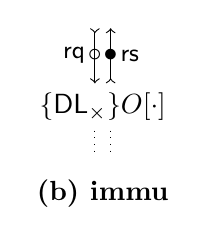
\begin{tikzpicture}
        \draw [<-<] (-0.1, 0.1) -- (-0.1, 0.8);
        \draw [>->] (0.1, 0.1) -- (0.1, 0.8);
        \node at (0, -0.2) {$\ppo{\dlfree{}}{O}{\cdot}$};
        \draw [dotted] (-0.1, -0.5) -- (-0.1, -0.8);
        \draw [dotted] (0.1, -0.5) -- (0.1, -0.8);
        \node[label={[label distance=-6pt]left:{\small {\sf rq}}}] at (-0.1, 0.45) {$\circ$};
        \node[label={[label distance=-6pt]right:{\small {\sf rs}}}] at (0.1, 0.45) {$\bullet$};
        \node at (0, -1.3) {{\bf (b) immu}};
      \end{tikzpicture}
    \end{adjustbox}&
    An immediate-up ({\bf immu}) rule responds immediately to a downward request, and it only requires the downlock free.
    In other words, even when uplocked, an object can make a state transition by taking a downward request and generating an upward response immediately.\\
  \end{tabular}
\end{center}

\paragraph{Rule templates to communicate with the parent}

\begin{center}
  \begin{tabular}{p{0.18\textwidth}p{0.77\textwidth}}
    \begin{adjustbox}{valign=t}
      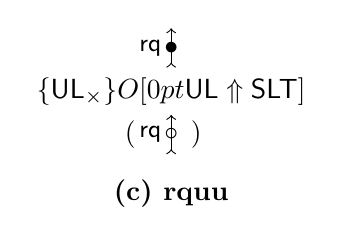
\begin{tikzpicture}
        \draw [>->] (0, 0.3) -- (0, 0.8);
        \node at (0, 0) {$\ppo{\ulfree{}}{O}{\bfrac{\setul{}}{\stsilent{}}}$};
        \draw [<-<] (0, -0.3) -- (0, -0.8);
        \node[label={[label distance=-6pt]left:{\small {\sf rq}}}] at (0, -0.55) {$\circ$};
        \node[label={[label distance=-6pt]left:{\small {\sf rq}}}] at (0, 0.55) {$\bullet$};
        \node at (-0.1, -0.55) {$(\qquad)$};
        \node at (0, -1.3) {{\bf (c) rquu}};
      \end{tikzpicture}
    \end{adjustbox}&
    A request-up-up ({\bf rquu}) rule (possibly) takes an upward request from a child and make another request to the parent.
    It requires the uplock to be free but does not care whether the object is downlocked or not.
    A state transition is not allowed when setting any lock (either an uplock or a downlock).
  \end{tabular}
\end{center}

\begin{center}
  \begin{tabular}{p{0.18\textwidth}p{0.77\textwidth}}
    \begin{adjustbox}{valign=t}
      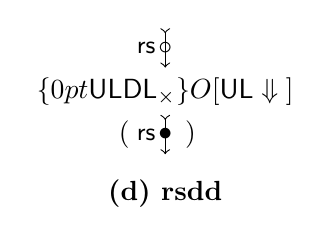
\begin{tikzpicture}
        \draw [<-<] (0, 0.3) -- (0, 0.8);
        \node at (0, 0) {$\ppo{\bfrac{\uled{}}{\dlfree{}}}{O}{\relul{}}$};
        \draw [>->] (0, -0.3) -- (0, -0.8);
        \node[label={[label distance=-6pt]left:{\small {\sf rs}}}] at (0, 0.55) {$\circ$};
        \node[label={[label distance=-6pt]left:{\small {\sf rs}}}] at (0, -0.55) {$\bullet$};
        \node at (-0.1, -0.55) {$(\qquad)$};
        \node at (0, -1.3) {{\bf (d) rsdd}};
      \end{tikzpicture}
    \end{adjustbox}&
    A response-down-down ({\bf rsdd}) rule is a dual of the {\bf rquu} rule, which takes a downward response and (possibly) responds to the original child requestor.
    This rule releases the corresponding uplock.
    Note that in order to handle a response from the parent, the object should be downlock-free.
    This precondition is indeed required to ensure correctness (serializability), as explained in \autoref{sec-locking-mechanism}.
  \end{tabular}
\end{center}

\paragraph{Rule templates to communicate with children}

\begin{center}
  \begin{tabular}{p{0.18\textwidth}p{0.77\textwidth}}
    \begin{adjustbox}{valign=t}
      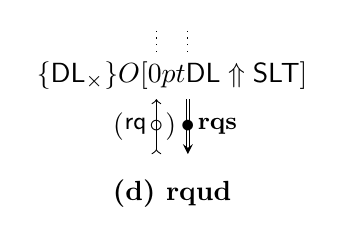
\begin{tikzpicture}
        \draw [dotted] (-0.2, 0.5) -- (-0.2, 0.8);
        \draw [dotted] (0.2, 0.5) -- (0.2, 0.8);
        \node at (0, 0.2) {$\ppo{\dlfree{}}{O}{\bfrac{\setdl{}}{\stsilent{}}}$};
        \draw [<-<] (-0.2, -0.1) -- (-0.2, -0.8);
        \draw [>=stealth,double,->] (0.2, -0.1) -- (0.2, -0.8);
        \node[label={[label distance=-6pt]left:{\small {\sf rq}}}] at (-0.2, -0.45) {$\circ$};
        \node[label={[label distance=-6pt]right:{\small {\sf {\bf rqs}}}}] at (0.2, -0.45) {$\bullet$};
        \node at (-0.35, -0.45) {$(\enspace\quad)$};
        \node at (0, -1.3) {{\bf (d) rqud}};
      \end{tikzpicture}
    \end{adjustbox}&
    A request-up-down ({\bf rqud}) rule (possibly) takes an upward request and makes downward requests to some of the children except the child requestor.
    A downlock is set in this case, and thus no state transition is allowed.
    This rule does not have a precondition that the object should be uplock-free, \ie{} the object can handle a request from the parent even when uplocked.
    This relaxation is still safe in terms of correctness (serializability) and necessary to avoid a deadlock.
  \end{tabular}
\end{center}

\begin{center}
  \begin{tabular}{p{0.18\textwidth}p{0.77\textwidth}}
    \begin{adjustbox}{valign=t}
      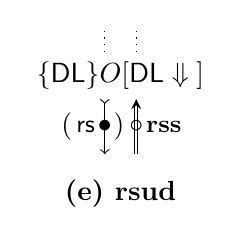
\begin{tikzpicture}
        \draw [dotted] (-0.2, 0.5) -- (-0.2, 0.8);
        \draw [dotted] (0.2, 0.5) -- (0.2, 0.8);
        \node at (0, 0.2) {$\ppo{\dled{}}{O}{\reldl{}}$};
        \draw [>->] (-0.2, -0.1) -- (-0.2, -0.8);
        \draw [>=stealth,double,<-] (0.2, -0.1) -- (0.2, -0.8);
        \node[label={[label distance=-6pt]left:{\small {\sf rs}}}] at (-0.2, -0.45) {$\bullet$};
        \node[label={[label distance=-6pt]right:{\small {\sf {\bf rss}}}}] at (0.2, -0.45) {$\circ$};
        \node at (-0.35, -0.45) {$(\enspace\quad)$};
        \node at (0, -1.3) {{\bf (e) rsud}};
      \end{tikzpicture}
    \end{adjustbox}&
    A response-up-down ({\bf rsud}) rule is a dual of the {\bf rqud} rule, which takes upward responses and (possibly) responds back to the original child requestor.
    The rule releases the corresponding downlock.
    As explained in \autoref{sec-locking-mechanism}, it does not require any conditions on the uplock.
  \end{tabular}
\end{center}

\begin{center}
  \begin{tabular}{p{0.18\textwidth}p{0.77\textwidth}}
    \begin{adjustbox}{valign=t}
      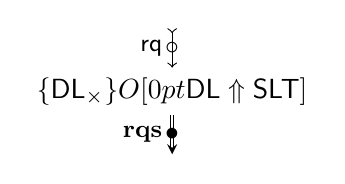
\begin{tikzpicture}
        \draw [<-<] (0, 0.3) -- (0, 0.8);
        \node at (0, 0) {$\ppo{\dlfree{}}{O}{\bfrac{\setdl{}}{\stsilent{}}}$};
        \draw [>=stealth,double,->] (0, -0.3) -- (0, -0.8);
        \node[label={[label distance=-6pt]left:{\small {\sf rq}}}] at (0, 0.55) {$\circ$};
        \node[label={[label distance=-6pt]left:{\small {\sf {\bf rqs}}}}] at (0, -0.55) {$\bullet$};
      \end{tikzpicture}
    \end{adjustbox}&
    A request-down-down ({\bf rqdd}) rule takes a downward request (from the parent) and makes downward requests to some of the children.
    Similar to {\bf rqud}, a downlock is set, and no state transition is allowed.
    This rule also does not require the object to be uplock-free, which is to avoid a deadlock.
  \end{tabular}
\end{center}

\begin{center}
  \begin{tabular}{p{0.18\textwidth}p{0.77\textwidth}}
    \begin{adjustbox}{valign=t}
      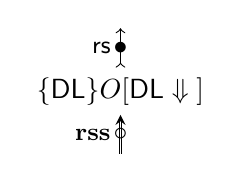
\begin{tikzpicture}
        \draw [>->] (0, 0.3) -- (0, 0.8);
        \node at (0, 0) {$\ppo{\dled{}}{O}{\reldl{}}$};
        \draw [>=stealth,double,<-] (0, -0.3) -- (0, -0.8);
        \node[label={[label distance=-6pt]left:{\small {\sf rs}}}] at (0, 0.55) {$\bullet$};
        \node[label={[label distance=-6pt]left:{\small {\sf {\bf rss}}}}] at (0, -0.55) {$\circ$};
      \end{tikzpicture}
    \end{adjustbox}&
    A response-up-up ({\bf rsuu}) rule is a dual of the {\bf rqdd} rule, which takes upward responses and responds back to the parent.
    Similar to {\bf rsud}, this rule also releases the corresponding downlock.
  \end{tabular}
\end{center}

\paragraph{A rule template for the whole-tree traversal}

\begin{center}
  \begin{tabular}{p{0.18\textwidth}p{0.77\textwidth}}
    \begin{adjustbox}{valign=t}
      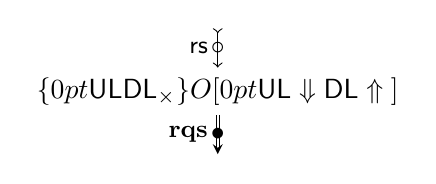
\begin{tikzpicture}
        \draw [<-<] (0, 0.3) -- (0, 0.8);
        \node at (0, 0) {$\ppo{\bfrac{\uled{}}{\dlfree{}}}{O}{\bfrac{\relul{}}{\setdl{}}}$};
        \draw [>=stealth,double,->] (0, -0.3) -- (0, -0.8);
        \node[label={[label distance=-6pt]left:{\small {\sf rs}}}] at (0, 0.55) {$\circ$};
        \node[label={[label distance=-6pt]left:{\small {\sf {\bf rqs}}}}] at (0, -0.55) {$\bullet$};
      \end{tikzpicture}
    \end{adjustbox}&
    A response-down-request-down rule ({\bf rsrq}) takes a downward response (from the parent) and makes new downward requests to some of the children.
    It makes a \emph{transfer} from an uplock to a new downlock by releasing the uplock and setting a downlock, where the child-requestor information is moved from the uplock.
    This rule forces the order of a traversal, saying that the traversal for the outer objects must be done before traversing the inner objects.
    The forced order is important to avoid a deadlock.
    For example, if the object makes requests to its parent and children at the same time and sets both an uplock and a downlock, a deadlock may occur.
  \end{tabular}
\end{center}

\paragraph{Remarks}

The rule templates are carefully designed to perform any practical transactions \emph{safely} with serializable behavior.
Consider an extreme case in a cache-coherence protocol.
When an L1 cache wants to obtain a write permission, all the other caches should be invalidated (changing each cache status to Invalid).
In order to perform such a transaction, it must be able to traverse all the other caches.
This transaction kind is one of the longest-running in cache-coherence protocols, and the rule templates are designed with proper locking ($\uled$ and $\dled$) and a state-change condition ($\stsilent$), not to create any incoherence while such a long transaction is interleaved with other transactions.

\chapter{Serializability Guarantee by \hemiola{}}

While conventional approaches to verifying cache-coherence protocols deal with transient states directly and induce noninterference lemmas per-state, \hemiola{} provides the serializability guarantee as \emph{the most general form of noninterference, obtained from conditions that are not coupled to any specific cache-coherence protocol}.

In order to satisfy such conditions for free, \hemiola{} limits protocols primarily by dictating network topologies and locking disciplines and by forcing rules to be defined using \emph{rule templates}.
We will present how the network topologies and the rule templates look and explain the intuition why using these components implies serializability, and we will sketch the actual proof using a technique called \emph{commuting reductions}.

\section{The Intuition: Separation by Topology, Network, and Locks}

\section{The Formal Proof of Serializability}

\subsection{Semi-sequential histories}

\subsection{Reduction of external input/output labels}

\subsection{Interleaving and nonconfluent histories}

\subsection{Reduction of atomic-history fragments}

\subsection{Serializability guarantee by \hemiola{}}

\chapter{Related Work I: Approaches to Dealing with Interleavings}
\label{sec-related-work-i}
